\documentclass{standalone}
\usepackage{tikz}
\usetikzlibrary{positioning, shapes.geometric, arrows.meta}

% 1. Use the standard Computer Modern Sans Serif
\usepackage[T1]{fontenc}
\renewcommand{\familydefault}{\sfdefault}


\begin{document}

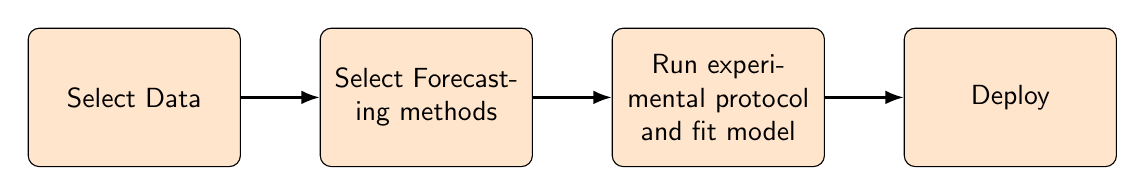
\begin{tikzpicture}[
    % Define the style for the boxes
    block/.style={
        rectangle, 
        draw, 
        fill=orange!20, 
        text width=7em, 
        text centered, 
        rounded corners, 
        minimum height=5em
    },
    % Define the style for the arrows
    line/.style={
        draw, 
        -Latex, 
        thick
    }
]

    % Place the nodes (boxes)
    \node [block] (box1) {Select Data};
    \node [block, right=1cm of box1] (box2) {Select Forecasting methods};
    \node [block, right=1cm of box2] (box3) {Run experimental protocol and fit model};
    \node [block, right=1cm of box3] (box4) {Deploy};

    % Draw the arrows
    \path [line] (box1) -- (box2);
    \path [line] (box2) -- (box3);
    \path [line] (box3) -- (box4);

\end{tikzpicture}

\end{document}